\documentclass{article}

\title{Collaborative Multi-Season Evaluation of Annual Influenza Forecasting Models in the U.S.}

\author{Logan Brooks, Spencer Fox, Craig McGowan, Sasikiran Kandula, \\ Dave Osthus, Evan Ray, Nicholas G Reich, Roni Rosenfeld, Jeffrey Shaman, \\Abhinav Tushar, Teresa Yamana [authorship list to be finalized]}

\usepackage[letterpaper, margin=1in]{geometry} % margin
\usepackage{lineno}% add line numbers
\usepackage{graphicx}
\usepackage[colorlinks=true, allcolors=blue]{hyperref}
\usepackage{parskip}        % for spacing after paragraphs http://ctan.org/pkg/parskip
\usepackage{url}            % simple URL typesetting
\usepackage{booktabs}       % professional-quality tables
\usepackage{amsfonts}       % blackboard math symbols
\usepackage{nicefrac}       % compact symbols for 1/2, etc.
\usepackage{amsmath, amsfonts}
\usepackage{setspace}
\linenumbers % line numbers
\onehalfspacing



% For computer modern sans serif
\usepackage[T1]{fontenc}
\renewcommand*\familydefault{\sfdefault} %% Only if the base font of the document is to be sans serif


\usepackage{Sweave}
\begin{document}
\input{comparison-manuscript-concordance}

\maketitle

\tableofcontents


\begin{Schunk}
\begin{Sinput}
> scores <- read_csv("../../scores/scores.csv")
> models <- read_csv("../../model-forecasts/component-models/model-id-map.csv")
> targets <- read_csv("../../scores/target-multivals.csv")
> complete_models <- c(models$`model-id`[models$complete=="true"], "UTAustin-edm")
> compartment_models <- c("CU-EAKFC_SEIRS", "CU-EAKFC_SIRS", "CU-EKF_SEIRS", 
+     "CU-EKF_SIRS", "CU-RHF_SEIRS", "CU-RHF_SIRS", "LANL-DBM")
> ## define column with scores of interest
> SCORE_COL <- quo(`Multi bin score`)
> ## Create data.frame of boundary weeks of scores to keep for each target/season
> all_target_bounds <- read_csv("data/all-target-bounds.csv")
> ## Remove scores that fall outside of evaluation period for a given target/season
> scores_trimmed <- scores %>% 
+     dplyr::left_join(all_target_bounds, by = c("Season", "Target", "Location")) %>%
+     dplyr::filter(`Model Week` >= start_week_seq, `Model Week` <= end_week_seq)
> ## truncate lowest possible scores to -10, define target-type variable
> scores_adj <- scores_trimmed %>%
+     filter(Model %in% complete_models) %>%
+     ## if NA, NaN or <-10, set score to -10
+     mutate(score_adj = dplyr::if_else(is.nan(!!SCORE_COL) | is.na(!!SCORE_COL) , 
+         -10, 
+         !!SCORE_COL),
+         target_type = dplyr::if_else(Target %in% c("Season onset", "Season peak week", "Season peak percentage"),
+             "seasonal", "k-week-ahead")) %>%
+     mutate(
+         score_adj = dplyr::if_else(score_adj < -10 , -10, score_adj),
+         Location = factor(Location, levels=c("US National", paste("HHS Region", 1:10))),
+         model_type = ifelse(Model %in% compartment_models, "compartment_model", "stat_model"),
+         stat_model = ifelse(Model %in% compartment_models, 0, 1)
+         ) 
> scores_by_model <- scores_adj %>%
+     group_by(Model) %>%
+     summarize(
+         avg_logscore = mean(score_adj)
+     ) %>%
+     ungroup() %>%
+     mutate(Model = reorder(Model, avg_logscore))
> scores_by_model_target <- scores_adj %>%
+     group_by(Model, Target) %>%
+     summarize(
+         avg_logscore = mean(score_adj)
+     ) %>%
+     ungroup() %>%
+     mutate(Model = reorder(Model, avg_logscore))
> scores_by_model_season <- scores_adj %>%
+     group_by(Model, Season) %>%
+     summarize(
+         avg_logscore = mean(score_adj)
+     ) %>%
+     ungroup() %>%
+     mutate(Model = reorder(Model, avg_logscore))
> scores_by_model_targettype <- scores_adj %>%
+     group_by(Model, target_type) %>%
+     summarize(
+         avg_logscore = mean(score_adj)
+     ) %>%
+     ungroup() %>%
+     mutate(Model = reorder(Model, avg_logscore))
> scores_by_model_region <- scores_adj %>%
+     group_by(Model, Location) %>%
+     summarize(
+         avg_logscore = mean(score_adj)
+     ) %>%
+     ungroup() %>%
+     mutate(Model = reorder(Model, avg_logscore))
> scores_by_model_season_target <- scores_adj %>%
+     group_by(Model, Season, Target) %>%
+     summarize(
+         avg_logscore = mean(score_adj)
+     ) %>%
+     ungroup() %>%
+     mutate(Model = reorder(Model, avg_logscore))
> scores_by_model_season_target_region <- scores_adj %>%
+     group_by(Model, Season, Target, Location) %>%
+     summarize(
+         avg_logscore = mean(score_adj)
+     ) %>%
+     ungroup() %>%
+     mutate(Model = reorder(Model, avg_logscore))
> scores_by_model_targettype_region <- scores_adj %>%
+     group_by(Model, target_type, Location) %>%
+     summarize(
+         avg_logscore = mean(score_adj)
+     ) %>%
+     ungroup() %>%
+     mutate(Model = reorder(Model, avg_logscore))
> scores_by_model_season_targettype_region <- scores_adj %>%
+     group_by(Model, Season, target_type, Location) %>%
+     summarize(
+         avg_logscore = mean(score_adj)
+     ) %>%
+     ungroup() %>%
+     mutate(Model = reorder(Model, avg_logscore))
> scores_by_region <- scores_adj %>%
+     group_by(Location) %>%
+     summarize(
+         avg_logscore = mean(score_adj)
+     ) %>%
+     ungroup() %>%
+     mutate(Location = reorder(Location, avg_logscore))
> scores_by_season <- scores_adj %>%
+     group_by(Season) %>%
+     summarize(
+         avg_logscore = mean(score_adj)
+     ) %>%
+     ungroup() %>%
+     mutate(Season = reorder(Season, avg_logscore))
> scores_by_region_targettype <- scores_adj %>%
+     group_by(Location, target_type) %>%
+     summarize(
+         avg_logscore = mean(score_adj)
+     ) %>%
+     ungroup() %>%
+     mutate(Location = reorder(Location, avg_logscore))
\end{Sinput}
\end{Schunk}



\section{Introduction}

In recent years, the quantity of research on forecasting infectious diseases has increased XX fold. 
This increased interest has been fueled in part by the promise of `big data', that near real-time data streams of large-scale population behavior \cite{Molodecky2017} to microscopic changes in a pathogen \cite{Du2017} could lead to measurable improvements in how disease transmission is measured, forecasted, and prevented \cite{Bansal2016}. 
With the spectre of a global pandemic looming, improving infectious disease forecasting continues to be a central priority of global health preparedness efforts.\cite{Myers2000,WHO2016}

Forecasts of infectious disease transmission can inform public health response to outbreaks. 
Accurate forecasts of the timing and spatial spread of seasonal outbreaks of diseases such as influenza or dengue fever can provide valuable information about where public health interventions can be targeted.
Decisions about hospital staffing, resource allocation, and the timing of public health communication campaigns could be assisted by forecasts. 
Implementation of interventions designed to disrupt disease transmissions, such as vector control measures or mandatory infection prevention protocols at hospitals or helath clinics, could be targeted based on forecasted incidence.

Public health officials are still learning how to best integrate forecasts into real-time decision making.
Close collaboration between public health policy-makers and quantitative modelers is necessary to ensure the forecasts have maximum impact and are appropriately communicated to the public and the broader public health community. 
Understanding what targets should be forecasted for maximum public health impact is hard to assess without real-time implementation and testing.


Starting in the 2013-2014 influenza season, the U.S. Centers for Disease Control and Prevention (CDC) has run the "Forecast the Influenza Season Collaborative Challenge" (a.k.a. FluSight) each influenza season, soliciting weekly forecasts for specific influenza season metrics from teams across the world.
These forecasts are displayed together on a website during the season and are evaluated for accuracy after the season is over.\cite{PhiResearchLab} 
This effort has galvanized a community of scientists interested in forecasting, creating an organic testbed for improving both our technical understanding of how different forecast models perform but also how to integrate these models into decsision-making.

Building on the structure of the FluSight challenges (and those of other collaborative forecasting efforts\cite{Viboud}), a subset of participants founded a consortium to facilitate direct comparison and fusion of modeling approaches. 
In this paper, we provide a detailed analysis of the performance of 22 different models from 5 different teams over the course of seven influenza seasons.
Drawing on the different expertise of the five teams allows us to make fine-grained and standardized comparisons of distinct modeling approaches that using different data sources.
Additionally, it allows us to identify gaps and continued challenges that should be addressed in future modeling efforts. 



% Infectious disease modeling has proven to be fertile ground for statisticians, mathematicians, and quantitative modelers for over a century. 
% Yet there is not a consensus on a single best modeling approach or method for forecasting the dynamic patterns of infectious disease outbreaks, in both endemic and emergent settings. 
% Mechanistic models consider the biological underpinnings of disease transmission, and are in practice are typically implemented as variations on the Susceptible-Infectious-Recovered (SIR) model. 
% Phenomenological models largely ignore the biological underpinnings and theory of disease transmission and focus instead on using data-driven, empirical and statistical approahces to make the best forecasts possible of a given dataset, or phenomenon. 
% Both approaches are commonly used and both have advantages and disadvantages in different settings.   


\section{Methods}

\subsection{FluSight Challenge Overview}
 
Detailed methodology and results from previous FluSight challenges have been published\cite{Biggerstaff2016}, but we summarize the key features of the challenge here.

The FluSight challenge focuses on forecasts of the weighted percentage of doctor's office visits for influenza-like-illness (wILI) in a particular region. 
This is a standard measure of seasonal flu activity, for which public data is available for the US back to the 1997/1998 influenza season. 
During each influenza season, this data is updated each week by the CDC (Figure \ref{fig:timezero-schematic}). When the most recent data is released, the prior weeks' reported wILI data may also be revised. 
The unrevised data, available at a particular moment in time, is available via the DELPHI real-time epidemiological data API beginning in the 2013/2014 season.\cite{DELPHI} 
This API enables researchers to ``turn back the clock'' to a particular moment in time and use the data available at that time. This enables more accurate assessment of how models would have performed in real-time. 

\begin{figure}[htbp]
\begin{center}
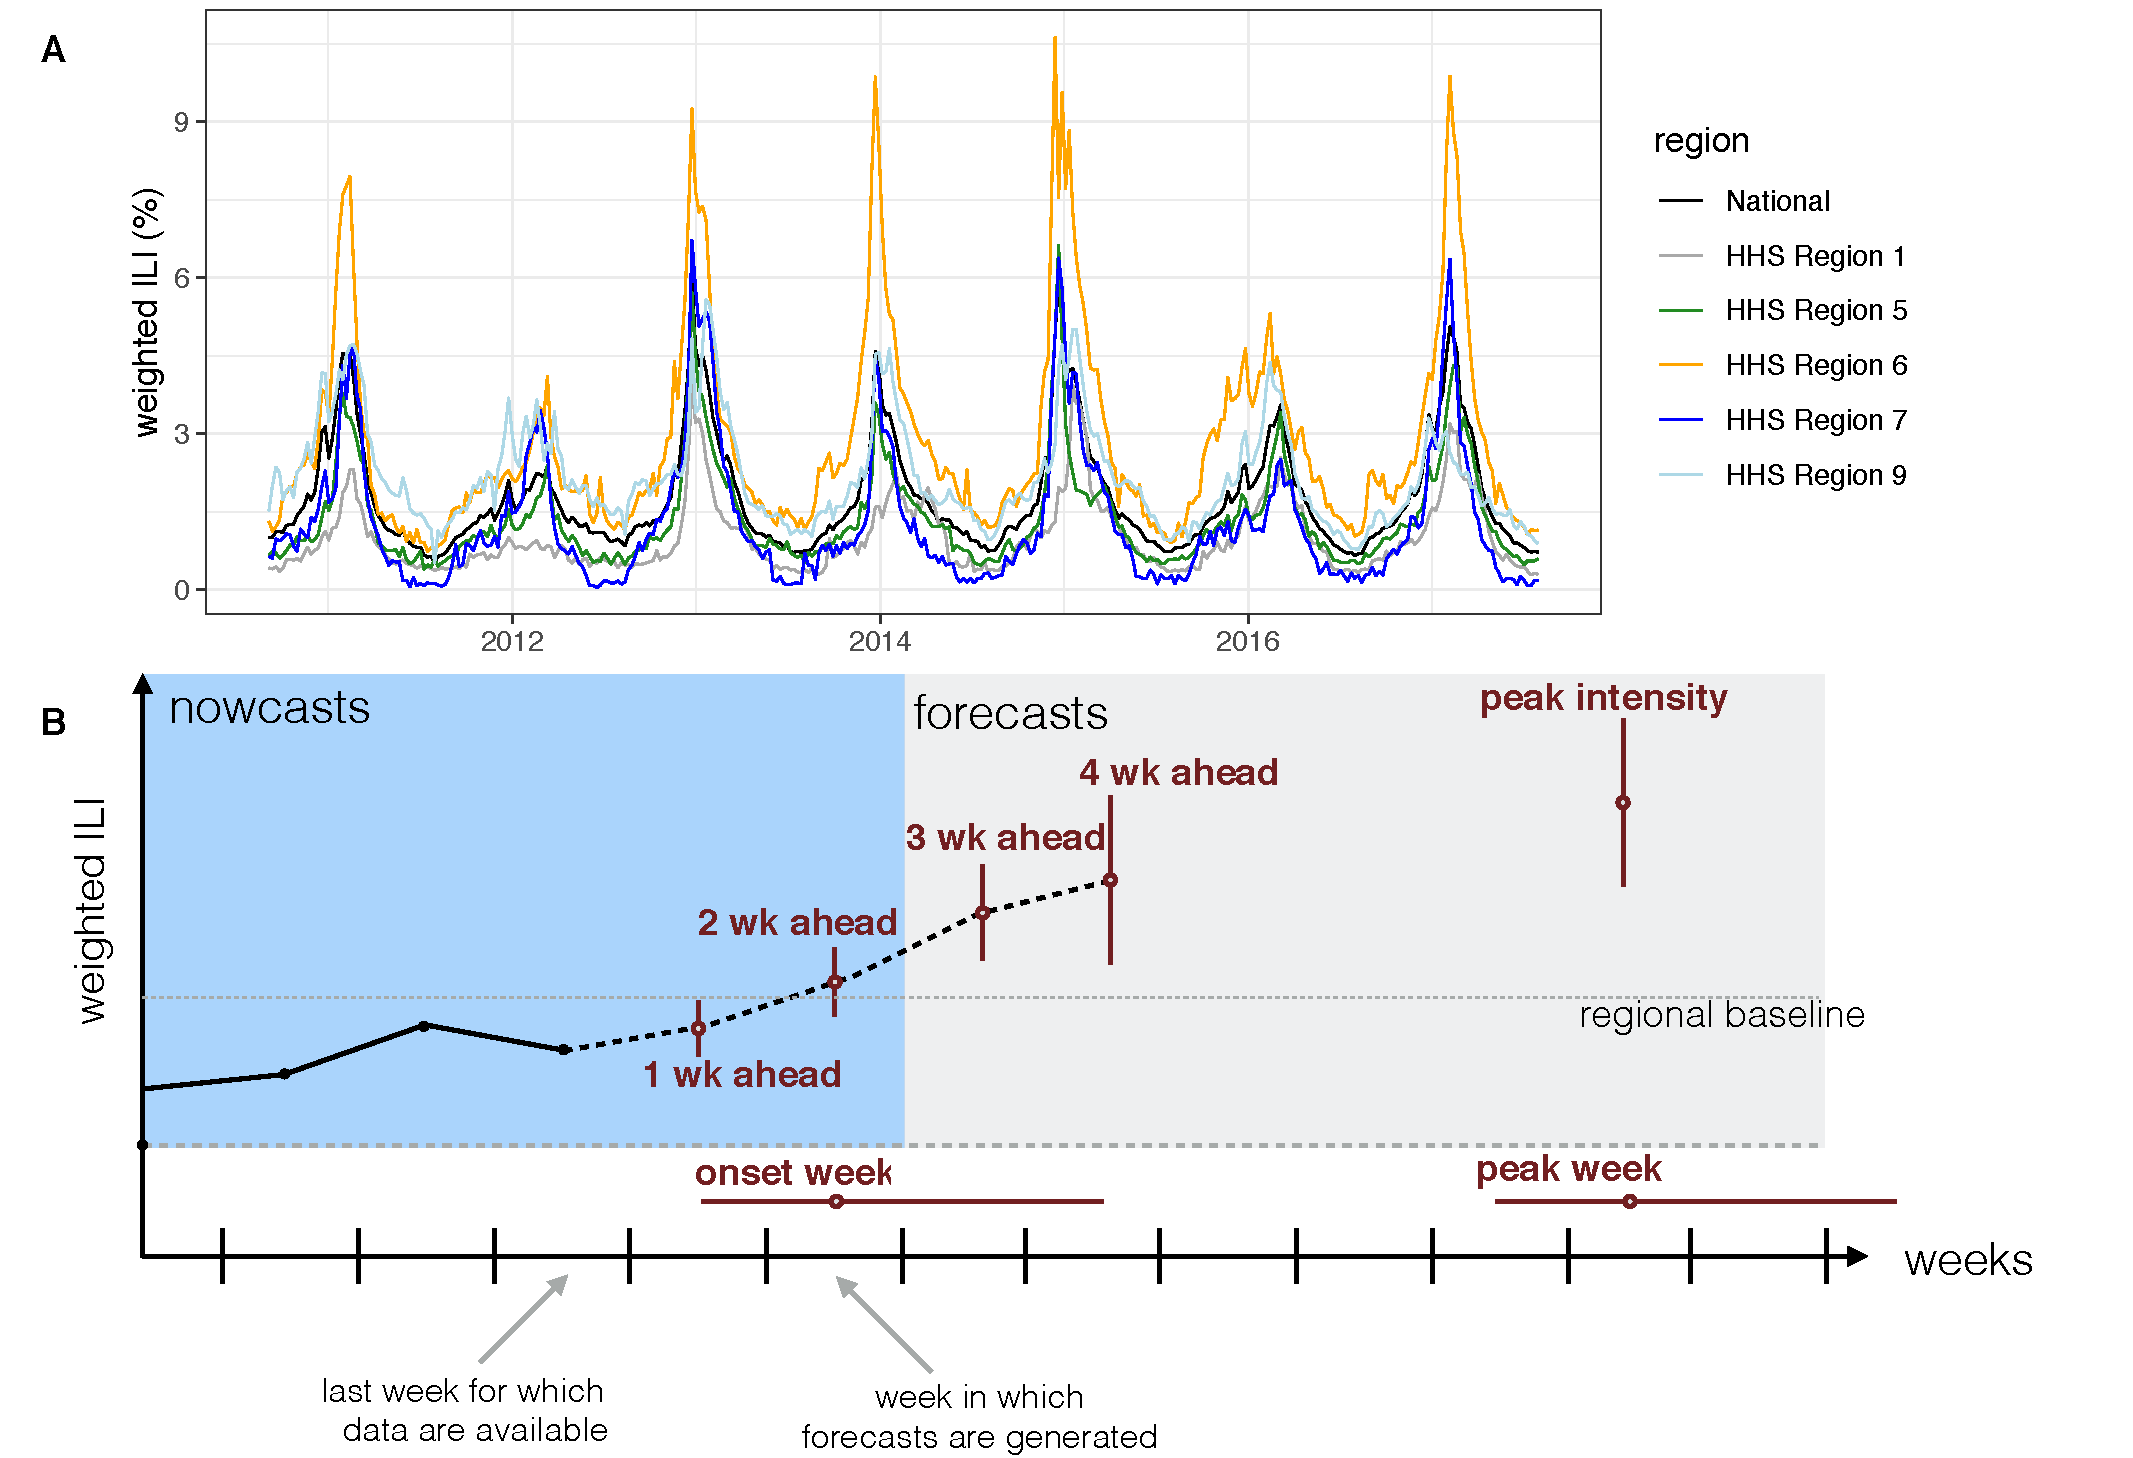
\includegraphics[width=\textwidth]{static-figures/timezero-sketch.pdf}
\caption{(A) Raw data weighted influenza-like illness data downloaded from the CDC website. The y-axis shows the weighted percentage of doctor's office visits for influenza-like illness for each week between September 2010 through July 2017, which is the time period for which the models presented in this paper made seasonal forecasts. (B) A diagram showing the anatomy of a single forecast. The seven forecasting targets are illustrated with a point estimate (dot) and interval (uncertainty bars). The five the targets on the wILI scale are shown with uncertainty bars spanning the vertical wILI axis, while the two targets for a time-of-year are illustrated with horizontal uncertainty bars along the temporal axis. The onset is defined relative to a region-specific baseline wILI percentage defined by the CDC. Arrows illustrate the timeline for a typical forecast for the CDC FluSight challenge, assuming that forecasts are generated or submitted to the CDC using the most recent reported data. This data includes the first reported observations of wILI\% from two weeks prior. Therefore, 1 and 2 week-ahead forecasts are considered nowcasts, i.e. at or before the current time. Similarly, 3 and 4 week-ahead forecasts are considered proper forecasts, or estimates about events in the future.}
\label{fig:intro-schematic}
\end{center}
\end{figure}


\begin{Schunk}
\begin{Sinput}
> ## code for plot in Figure 1
> regionflu <- get_flu_data("hhs", sub_region=1:10, data_source="ilinet", years=1997:2017)
> usflu <- get_flu_data("national", sub_region=NA, data_source="ilinet", years=1997:2017)
> ## make AGE cols in usflu integer data type
> cols <- grepl('^AGE', colnames(regionflu))
> regionflu[,cols] <- sapply(regionflu[,cols], as.integer)
> cols <- grepl('^AGE', colnames(usflu))
> usflu[,cols] <- sapply(usflu[,cols], as.integer)
> fludata <- bind_rows(regionflu, usflu)
> fludata <- dplyr::transmute(fludata,
+     region.type = `REGION TYPE`,
+     region = REGION,
+     year = YEAR,
+     week = WEEK,
+     caldate = as.POSIXct(MMWRweek2Date(YEAR, WEEK)),
+     weighted_ili = as.numeric(`% WEIGHTED ILI`))
> fludata$region[fludata$region == "X"] <- "National"
> fludata$region <- factor(fludata$region, 
+     levels=c("National", paste("Region", 1:10)),
+     labels=c("National", paste("HHS Region", 1:10)))
> fludata %>%
+     filter(
+         region %in% c("National", paste("HHS Region", c(1,5,6,7,9))),
+         caldate > as.POSIXct(as.Date("2010-09-01")),
+         caldate < as.POSIXct(as.Date("2017-08-01"))) %>%
+     ggplot(aes(x=caldate, y=weighted_ili, color=region)) + 
+     xlab(NULL) + ylab("weighted ILI (%)") +
+     geom_line() +
+     scale_color_brewer(palette="Dark2")
\end{Sinput}
\end{Schunk}


The FluSight challenges have defined seven forecasting targets of particular public health relevance. Three of these targets are fixed scalar values for a particular season: onset week, peak week, and peak intensity (i.e. the maximum observed wILI percentage). The remaining four targets are the observed wILI percentages in each of the subsequent four weeks (Figure \ref{fig:intro-schematic}). 

The FluSight challenges have also required that all forecast submissions and follow a particular format. A single submission file (a comma-separated text file) contains the forecast made for a particular epidemic week (EW) of a season. Standard CDC definitions of epidemic week are used. Each file contains binned predictive distributions for seven specific targets across the 10 HHS regions of the US plus the national level. Each file contains over 8000 rows and typically is about 400KB in size.

To be included in the model comparison presented here, previous participants in the CDC FluSight challenge were invited to provide out-of-sample forecasts for the 2010/2011 through 2016/2017 seasons. For each model, this involved creating 233 separate forecast submission files, one for each of the weeks in the seven training seasons.
Each forecast file represented a single submission file, as would be submitted to the CDC challenge. 
Each team created their submitted forecasts in a prospective, out-of-sample fashion, i.e. fitting or training the model only on data available before the time of the forecast (see Figure \ref{fig:intro-schematics}). 

\subsection{Summary of Models}

Five teams each submitted between 1 and 9 separate models for evaluation (Table \ref{tab:model-list}). 
A wide range of methodological approaches and modeling paradigms are included in the set of forecast models.
For example, seven of the models utilize a compartmental structure (e.g. Susceptible-Infectious-Recovered), a model framework that directly encodes both the transmission and the susceptible-limiting dynamics of infectious disease outbreaks.
Other less directly mechanistic models use statistical approaches to model the outbreak phenomenon directly by incorporating recent incidence and seasonal trends.
[[Six]] models directly incorporate external data (i.e. not just the wILI measurements from the CDC ILINet dataset), including historical humidity data and Google search data.
Two models stand out as being clear na\"ive baseline models, that never change based on recent data. 
The {\tt Delphi-Uniform} model always provides a forecast that assigns equal probability to all possible outcomes. 
The {\tt ReichLab-KDE} model yields predictive distributions based entirely on data from other seasons using kernel density estimation (KDE) for seasonal targets and a generalized additive model with cyclic penalized splines for weekly incidence.
Throughout the manuscript when we refer to the `historical baseline` model we mean the {\tt ReichLab-KDE} model.
Once submitted to the central repository, the models were not updated or modified except in [[XX]] cases to fix explicit bugs in the code that unearthed numerical problems with the forecasts. 
Re-fitting of models or tuning of model parameters was explicitly discouraged and disallowed to avoid unintentional overfitting of models.

\begin{table}
\setlength{\tabcolsep}{4pt} 
\begin{tabular}{p{1.69cm} l p{7.5cm}  p{1.70cm}  p{1.7cm}}
\hline
Team     & Model Abbr& Model Description & External Data & Comp. Model* \\ 
\hline
CU       & EAKFC\_SEIRS       & Ensemble Adjustment Kalman Filter SEIRS                                                        & x             & x                   \\ 

~        & EAKFC\_SIRS        & Ensemble Adjustment Kalman Filter SIRS                                                         & x             & x                   \\
~        & EKF\_SEIRS         & Ensemble Kalman Filter SEIRS                                                                   & x             & x                   \\
~        & EKF\_SIRS          & Ensemble Kalman Filter SIRS                                                                    & x             & x                   \\
~        & RHF\_SEIRS         & Rank Histogram Filter SEIRS                                                                    & x             & x                   \\
~        & RHF\_SIRS          & Rank Histogram Filter SIRS                                                                     & x             & x                   \\
~        & BMA                & Bayesian Modeling Average                                                                      & ~             & ~                   \\
\hline
Delphi   & BasisRegression    & Basis Regression (epiforecast package defaults)                                                & ~             & ~                   \\ 
~        & DeltaDensity1      & Delta Density (epiforecast package defaults)                                                   & ~             & ~                   \\ 
~        & EmpiricalBayes1    & Empirical Bayes (conditioning on past four weeks only)                                         & ~             & ~                   \\ 
~        & EmpiricalBayes2    & Empirical Bayes (epiforecast package defaults)                                                 & ~             & ~                   \\ 
~        & EmpiricalFuture    & Empirical Futures (epiforecast package defaults)                                               & ~             & ~                   \\ 
~        & EmpiricalTraj      & Empirical Trajectories (epiforecast package defaults)                                          & ~             & ~                   \\ 
~        & DeltaDensity2      & Markovian Delta Density (epiforecast package defaults)                                         & ~             & ~                   \\ 
~        & Stat               & Statistical Ensemble (using the eight submitted components, with no backcasting or nowcasting) & ~             & ~                   \\
~        & Uniform            & Uniform Distribution                                                                           & ~             & ~                   \\ 
\hline
LANL     & DBM                & Dynamic Bayesian Model with a hierarchical discrepancy                                         & ~             & x                   \\ 
\hline
ReichLab & KCDE               & Kernel Conditional Density Estimation                                                          & ~             & ~                   \\ 
~        & KDE                & Kernel Density Estimation                                                                      & ~             & ~                   \\ 
~        & SARIMA1            & SARIMA model without seasonal differencing                                                     & ~             & ~                   \\ 
~        & SARIMA2            & SARIMA model with seasonal differencing                                                        & ~             & ~                   \\ 
\hline
UTAustin & EDM                & Empirical Dynamic Model                                                                        & ~             & ~                   \\ 
\end{tabular}
\caption{List of models, with key characteristics. *Comp. model stands for compartmental model.}
\label{tab:model-list}
\end{table}

\subsection{Metric Used for Evaluation and Comparison}

Influenza forecasts have been evaluated by the CDC primarily using the log-score, a measure that enables evaluation of both the precision and accuracy of a forecast.\cite{Gneiting2007} 
The log-score is defined as $\log f(\hat z|\bf{x})$ where $f(z|\bf{x})$ is the predicted density function for some target $Z$, conditional on some data $\bf{x}$ and $\hat z$ is the observed value of the target $Z$. 
The log-score is a ``proper`` scoring rule, which has the practical implication that linear combinations (i.e. arithmetic means) of log scores will [[preserve overall rankings of forecasts]].


Consistent with the primary evaluation performed by the CDC, we used a modified form of the log-score to evaluate forecasts. 
The modified log-scores are computed for the targets on the wILI percentage scale such that predictions within +/- 0.5 percentage points are considered accurate, i.e. log score = $\log \int_{\hat z -.5}^{\hat z + .5} f^{(m)}(z|{\bf{x}})dz$. 
For the targets on the scale of epidemic weeks, predictions within +/- 1 week are considered accurate, i.e. log score = $\log \int_{\hat z -1}^{\hat z + 1} f^{(m)}(z|{\bf{x}})dz$. 
While this modification means that the resulting score is not formally a proper scoring rule, some have suggested that improper scores derived from proper scoring rules may, with large enough sample size, have negligible differences in practice.\cite{Gneiting2007} % see especially last paragraph of section 2.3 
Additionally, this modified log score has the advantage of having a clear interpretation motivated and designed by public health officials.
Hereafter, we will refer to these modified log scores as simply log scores.

Average log scores can be used to compare models' performance in forecasting for different locations, seasons, targets, or times of year.
In practice, each model $m$ has a set of log scores associated with it are region-, target-, season-, and week-specific.
We represent one specific scalar log score value as $\log f_{m,r,t,s,w}(\hat z|\bf{x})$. 
These values can be averaged across any of the indices to create a summary measure of performance.
For example,
\begin{eqnarray}
LS_{m,\cdot,t,\cdot,\cdot} & = & \frac{1}{N} \sum_{r,s,w} \log \hat f_{m,r,t,s,w}(\hat z|{\bf x})
\end{eqnarray}
represents a log score for model $m$ and target $t$ averaged across all regions, seasons and weeks.

While log scores are not on a particularly interpretable scale, a simple transformation enhances interpretability substantially.
Exponentiating an average log score yields a forecast score equivalent to the geometric mean of the probabilities assigned to the eventually observed outcome. 
The geometric mean is an alternative measure of central tendency to an arithmetic mean, representing the $n^{th}$ root of a product of $n$ numbers. 
Using the example above, we then have that
\begin{eqnarray}
S_{m,\cdot,t,\cdot,\cdot} = \exp \left ( LS_{m,\cdot,t,\cdot,\cdot} \right } & = & \exp \left ( \frac{1}{N} \sum_{r,s,w} \log \hat f_{m,r,t,s,w}(\hat z|{\bf x}) \right ) \\
 & = & \left ( \prod_{r,s,w} \hat f_{m,r,t,s,w}(\hat z|{\bf x}) \right ) ^{1/N} 
\end{eqnarray}
In this setting, this score has the intuitive interpretation of being the average probability assigned to the true outcome (where average is considered to be a geometric average).
Hereafter, we will refer to an average score as an exponentiated average log score.
In all cases, we compute the averages arithmetically on the log scale and only exponentiate before reporting and interpreting a final number.

Following the convention of the CDC challenges, we only included certain weeks in the calculation of the average log scores for each target.
Forecasts of season onset are evaluated based on the forecasts that are received up to six weeks after the observed onset week within a given region.
Forecasts of season peak and intensity are evaluated through the first forecast received after the weighted ILI goes below the regional baseline for the final time during a given region-season. 
Week-ahead forecasts are evaluated using forecasts received four weeks prior to the onset week through forecasts received three weeks after the weighted ILI goes below the regional baseline for the final time.
In a region-season without an onset, all weeks are scored.
To ensure all calculated summary measures would be finite, all modified log scores with values of less than -10 were assigned the value -10, following CDC scoring conventions.

\subsection{Formal comparisons of model performance}

Model-based comparisons of forecast accuracy are hindered by the high correlation of sequential forecasts and by outlying observations. 
When observations assign no probability to the eventually observed outcome they have a log-score of $-\infty$.

%Things to confirm: removed weeks that CDC does not score, no onset seasons and multi peak years are handled appropriately

\subsection{Analysis of delays}
[GLM regression model with ...]

\section{Results}

\subsection{Comparing models' forecasting performance by season}
\begin{Schunk}
\begin{Sinput}
> kde_logscore <- unlist(scores_by_model[which(scores_by_model$Model=="ReichLab-KDE"), "avg_logscore"])
> max_logscore <- max(scores_by_model$avg_logscore)
> min_logscore <- min(scores_by_model$avg_logscore)
> max_logscore_model <- as.character(unlist(scores_by_model[which(scores_by_model$avg_logscore == max_logscore), "Model"]))
> min_logscore_model <- as.character(unlist(scores_by_model[which(scores_by_model$avg_logscore == min_logscore), "Model"]))
> n_above_kde <- sum(scores_by_model$avg_logscore>kde_logscore)
> n_models <- nrow(scores_by_model)
> n_seasons <- nrow(scores_by_season)
> n_regions <- nrow(scores_by_region)
> tmp <- scores_by_model_season %>% group_by(Model) %>%
+     summarize(n_seasons_above_maxavg = sum(avg_logscore>max_logscore)) 
\end{Sinput}
\end{Schunk}


Averaging across targets and locations, forecast skill varied widely by model and season (Figure \ref{fig:results-model-season}). 
The historical baseline model showed an average seasonal skill of 
0.20, 
meaning that in an typical season, across all targets and locations, this model assigned on average 
0.20 
probability to the eventually observed value. 
The model with the highest average seasonal forecast skill 
({\tt Delphi-Stat}) 
and lowest 
({\tt Delphi-EmpiricalBayes2}) 
had scores of 0.37 and 0.07, respectively. 
Of the 22 models, 16 models 
(73\%) 
showed higher average seasonal forecast skill than the historical average.
Season-to-season variation was substantial, with 
10 
models having at least one season with greater average forecast skill than the best model did.

